\documentclass{article}
\usepackage{graphicx} % Required for inserting images
\usepackage[english]{babel} % English formatting
\usepackage[utf8]{inputenc} % Standard encoding
\usepackage[a4paper,left=4cm,bottom=2cm]{geometry} % Page formatting
\usepackage{indentfirst} % Indents the first paragraph
\usepackage{amsmath} % Maths type package
\usepackage{bm} % Bold font maths
\usepackage{graphicx} % Advanced graphics package
\usepackage[export]{adjustbox} 
\usepackage{fancyhdr} % Fancy headers
\usepackage{hyperref}
\usepackage{amsthm}
\usepackage{cleveref}
\usepackage{bm}
\usepackage{wrapfig} % Text flowing around figures

\newtheorem{thm}{Theorem}[section]
\newtheorem{cor}[thm]{Corollary}
\newtheorem{prop}[thm]{Proposition}
\newtheorem{lem}[thm]{Lemma}
\newtheorem{conj}[thm]{Conjecture}
\newtheorem{quest}[thm]{Question}
\newtheorem{claim}[thm]{Claim}
\newtheorem{ppty}[thm]{Property}

\theoremstyle{definition}
\newtheorem{defn}[thm]{Definition}
\newtheorem{defns}[thm]{Definitions}
\newtheorem{con}[thm]{Construction}
\newtheorem{exmp}[thm]{Example}
\newtheorem{exmps}[thm]{Examples}
\newtheorem{notn}[thm]{Notation}
\newtheorem{notns}[thm]{Notations}
\newtheorem{addm}[thm]{Addendum}
\newtheorem{exer}[thm]{Exercise}
\newtheorem{limit}[thm]{Limitation}


\theoremstyle{remark}
\newtheorem{rem}[thm]{Remark}
\newtheorem{rems}[thm]{Remarks}
\newtheorem{warn}[thm]{Warning}
\newtheorem{sch}[thm]{Scholium}

% \pagestyle{fancy}
% \fancyhf{}
\renewcommand{\footrulewidth}{0.4pt}

\title{Random CTLNs}
\author{Eric Han, Caitlin Lienkaemper}
\date{July-August 2024}

\begin{document}

\maketitle

\section{Project Summary}
The goal of this project was to observe the effects of symmetry in random combinatorial linear-threshold networks (CTLNs). The simulation model was built in Python. A major step taken this summer was the completion of a small but complete program to generate averaged heatmaps of how network dynamics behaved across various probability parameters. Additionally, at the tail-end of the project, a more mathematically focused thrust to the problem was conceptualized and a more concrete vision of tackling the symmetry problem was realized.

\section{Model}
The CTLN model is a simplified mathematical model of neural networks that focuses on the fine connectivity between neurons as the key factor affecting the resulting dynamics of the network. CTLNs exhibit strongly nonlinear dynamics, showcasing behavior such as multistability, chaotic attractors, and limit cycles. Physically, these models are similar to other classical attractor neural networks that model associative memory. For instance, the manifestation of limit cycles can indicate central pattern generators controlling periodic behaviors in animals. The main method of analysis for the CTLN model is through a graph theoretical lens. One can look directly at the structure and specific connectivity of the graph to determine the underlying dynamics of the network.



\section{Code}
\subsection{Algorithm}
The goal of this model is to generate random graphs with set parameters for symmetry and edge connection probability. This is done through the generation of a random square adjancency matrix of size $n$. Only the top diagonal of the matrix is generated with values of $\{-2,-1,1,2\}$. These values denote no edge, a unidirectional edge from $j$ to $i$, a unidirectional edge from $i$ to $j$, and a bidirectional edge between $j$ and $i$, respectively. The respective weight table for the values is $\{1-p, p(\frac{1-q}{2} ), p(\frac{1-q}{2} ), pq\}$, where $p$ denotes edge connection probability and $q$ is the symmetry parameter. As $q$ increases, general symmetry of the graph increases linearly.
\begin{defn}
Let $i,j$ be any two vertices with an edge between them in a directed graph. $i$ and $j$ are considered \textit{symmetric} if there exists a bidirectional edge between them. A graph is considered fully symmetric if every edge in the graph is a bidirectional edge; or if there exist no edges in the graph.
\end{defn}
A consequence of this generation method is that the generation of any bidirectional edge is controlled exclusively by the value $\{2\}$, that is, a bidirectional edge cannot be generated by the creation of 2 unidirectional edges in opposing direction between vertices $i$ and $j$.

\subsection{Application}
We use this algorithm to simulate dynamics for the full spectrum of edge connection probabilities and symmetry parametrizations. We generate random weight matrices for every unique combination of $p,q$. $p$ and $q$ are taken in intervals of $0.1$, but we do have the capacity for finer simulation. A stability analysis is included in the code but was ultimately too slow, as it attempted to analyze the stability of every node in the network.

\subsection{Heatmaps}
Due to the construction of the main algorithm, it is possible to generate heatmaps showcasing the average dynamics of single neurons. We use a threshold-based system to detect fixed points, that is, if the oscillation of the dynamics of a single neuron does not escape the bounds of $[-0.1,0.1]$ for a long timesecale $t=(0,600)$, $dt = 0.1$, we consider it a fixed point. More specifically, we observe the last 50 entries in the list of generated values using the RK4 method to see if the neuron's dynamics fall outside the threshold. If the dynamics fall outside the threshold, we consider it a non-fixed point. These non-fixed points may take the form of limit cycles, but from observation through simulation, they are more likely to be chaotic.

We assign a neuron that settles to a fixed point the value $k=1$. We assign a neuron that is \textit{not} a fixed point the value $k=0$. We take the average of all $k_{p,q}$ for all combinations of $p,q$.

We average the "fixed-point-edness" across 30 trials 7 times, for a total of 210 trials for a matrix of size $m$. A heatmap is generated in this method, using a spectrum for $\bar{k}_{p,q}$ from $[0,1]$.

\begin{figure}
    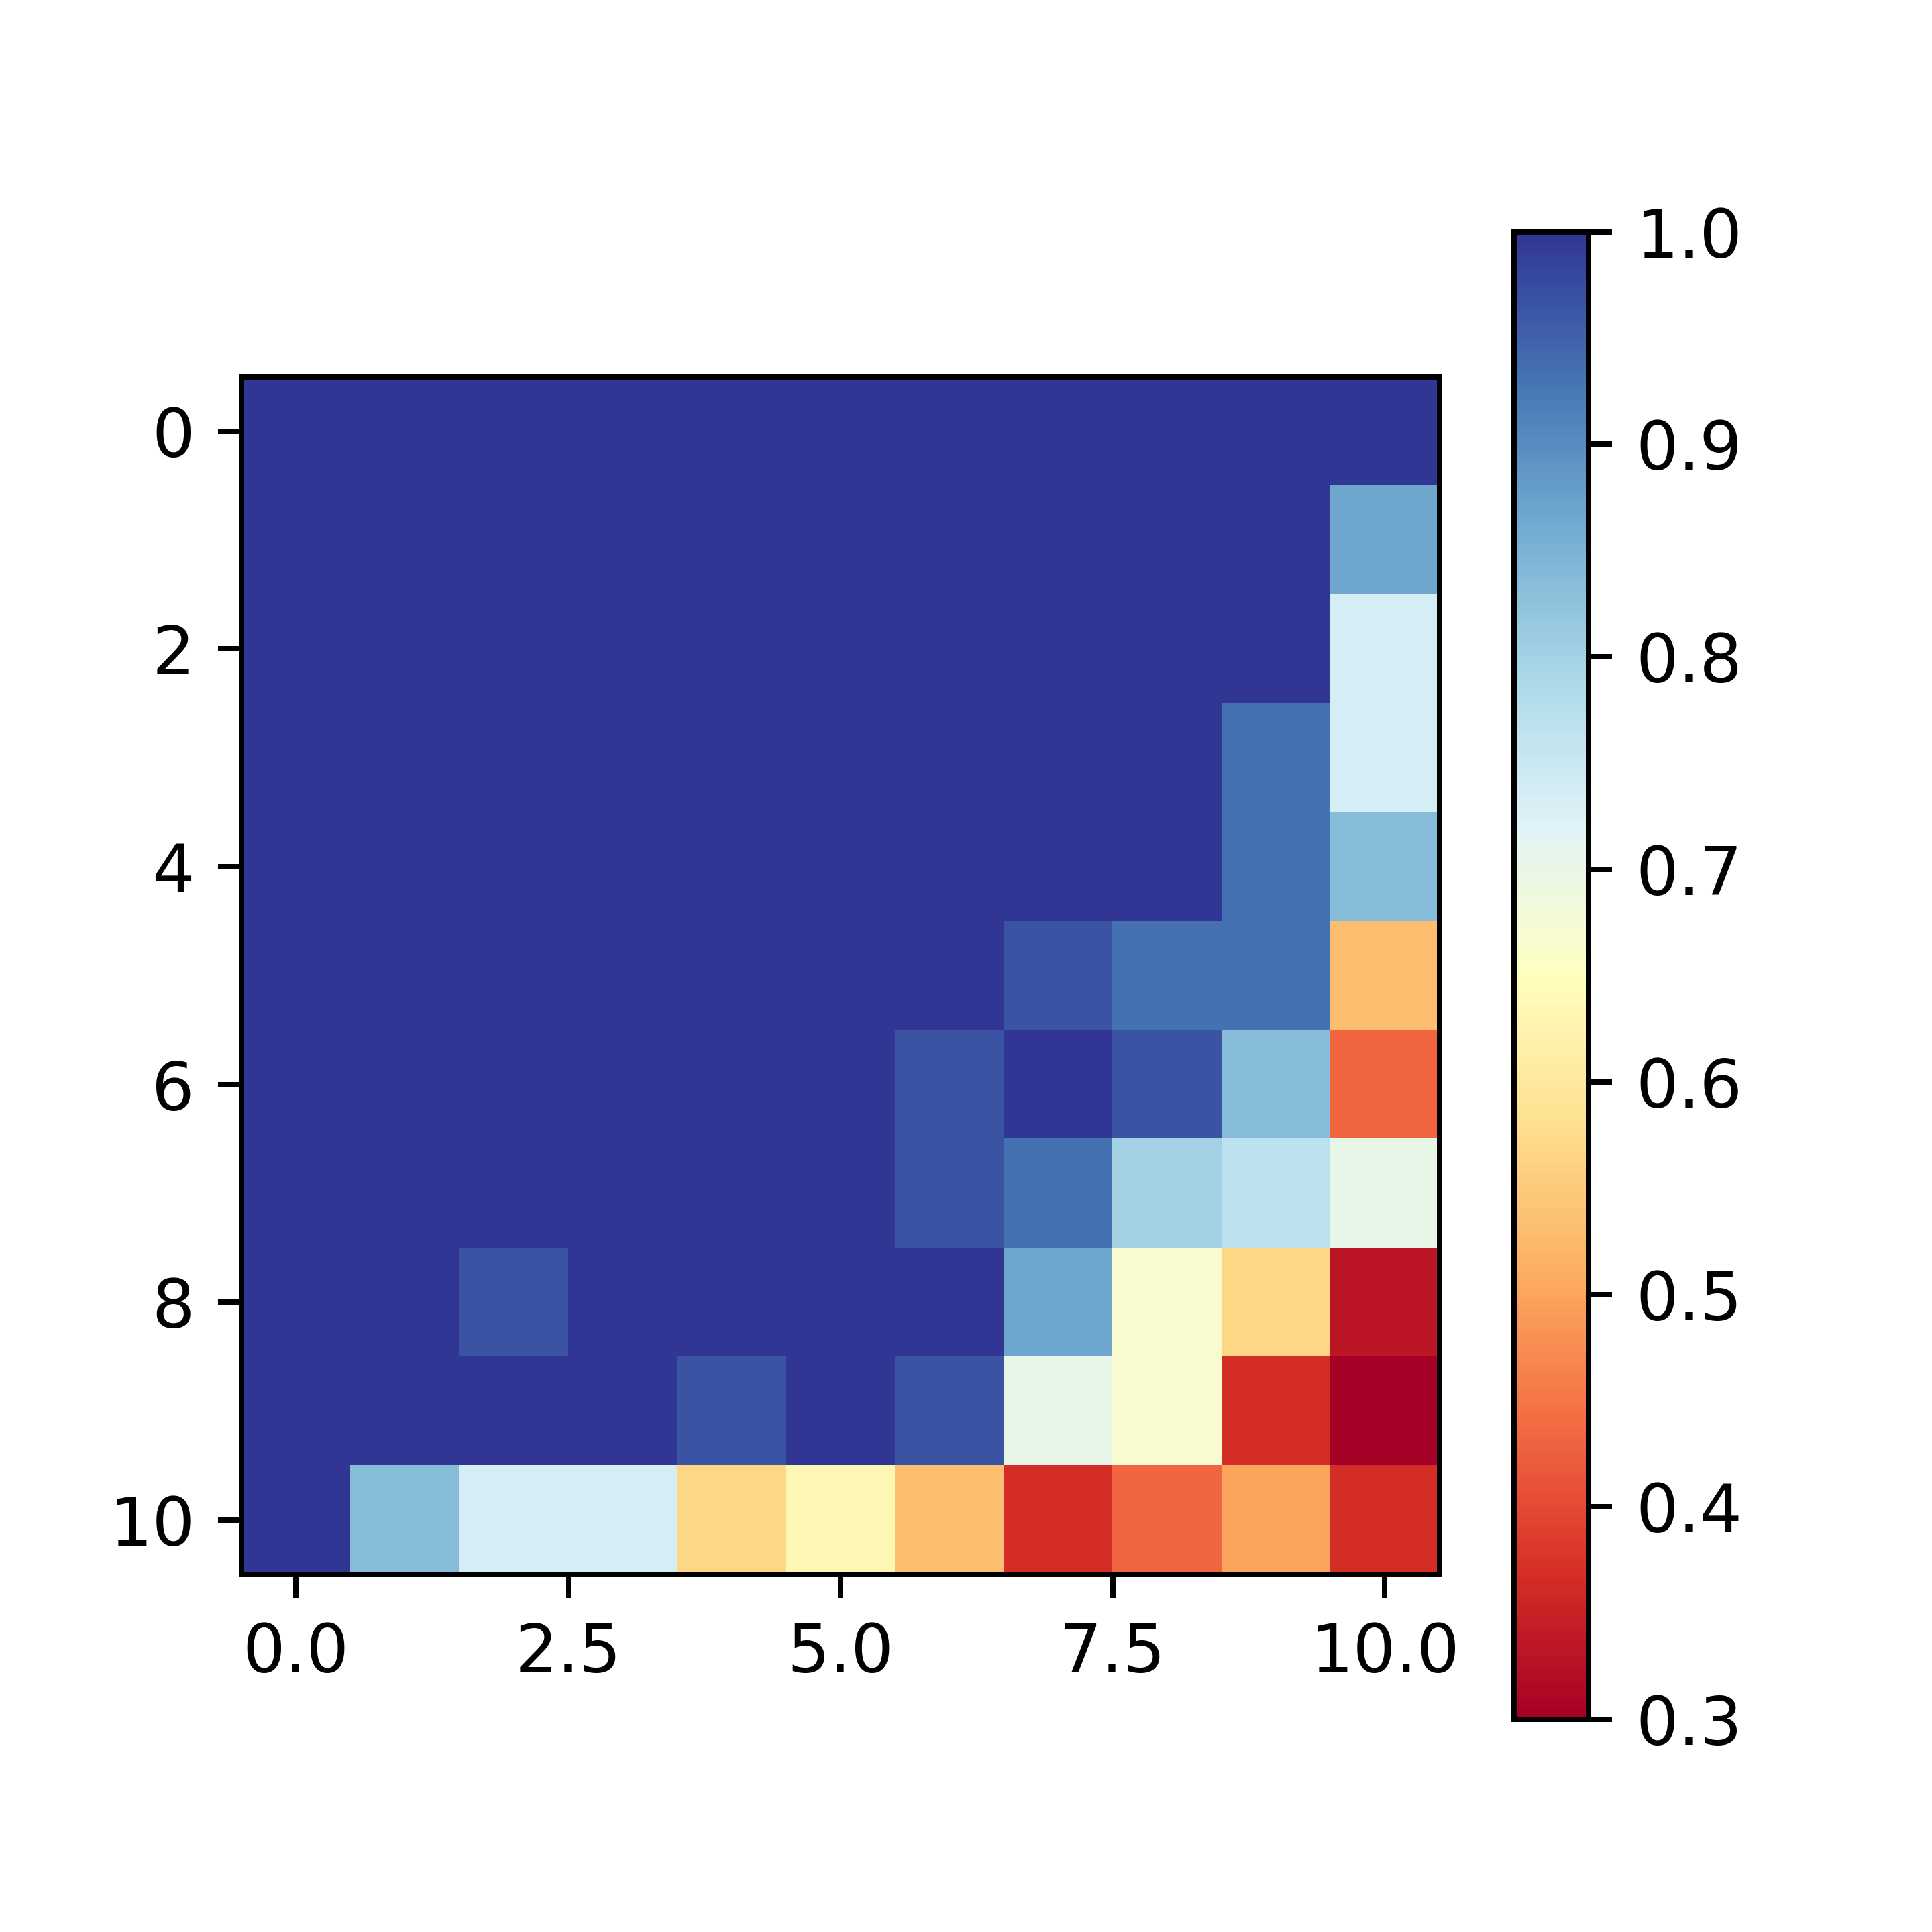
\includegraphics[width=3in]{Matrix Size 100 0.png}
    \caption{Heatmap for graph $n=100$}
\end{figure}

The central issue with this approach is the tolerance used to check whether a neuron settles to a fixed point. Because the energy in the system is shared amongst all firing neurons, the more neurons that exist, if the system is predisposed to being chaotic, the smaller the oscillations will be for every neuron. For large networks, these oscillations become small enough that non-fixed point neurons are marked as fixed points.

\section{Problem}
We are looking at the expected number of stable fixed points in any size $n$ graph by using the expected number of target free cliques as a function of the edge connection probability $p$ and the symmetry parameter $q$.

Because the CTLN model can be easily analyzed through a graph-theoretic lens, we aim to analyze stability through clique formation in a random graph. 

A recent, interesting result concerns the expected number of maximal cliques in any random $n$-sized graph. This is important because one can discern the dynamics of the graph through analyzing its graph structure. Because edge generation of our random graph is independent, that is, the generation of an edge does not have any impact on the generation of other edges, we can look for the probability of a single node in the graph destroying maximality.

\section{Key Definitions}  
\label{sec:Key Definitions}
\begin{defn}
    A \textit{clique} is defined as a subset of vertices on a graph such that every two distinct vertices in the clique share a bidirectional edge.
\end{defn}

\begin{defn}
    A \textit{maximal clique} is a clique that is not contained in a larger clique.
\end{defn}

\begin{defn}
    The \textit{target of a clique $\sigma$} is defined as a clique that receives an edge from every node in $\sigma$. A clique with no targets is called \textit{target-free}.
\end{defn}

A clique $\sigma$ is the support of a fixed point if and only if it is target free. That is, if the given clique is maximal, then it is a stable fixed point support.

\section{Findings}
\label{sec:Findings}
\begin{prop}
    Let E be the event that adding a node does not destroy maximality. Given the existence of a $k$-clique in a size $N$ Erd{\"o}s-Renyi graph, the probability that adding a node does not destroy maximality is given by
    \begin{align}
        \label{eq:e of max clique}
        P(E|k\text{-clique exists}) = (1-p^k)^{N-k}
    \end{align}
    where p is the edge connection probability.
\end{prop}
\begin{proof}
    Let $N$ denote the size of a random Erd{\"o}s-Renyi graph $G$. Let $p$ denote the edge connection probability of $G$. Let $\sigma_k\in G$ be any clique of size $k$ in $G$. Consider the probability of event $X$, being the event that adding any individual vertex $g_i\in G$ ruins the maximality of $\sigma_k$. The vertex would require an edge from every vertex in $\sigma_k$. For an edge connection with probability $p$ to be generated between every vertex in $\sigma_k$ and a single vertex $g$, we require $k$ edges to be independently drawn, obtaining the following result:
    \begin{align}
        \label{eq:}
        P \left(g \text{ ruins maximality}|\sigma_k \text{ exists} \right) = p^k.
    \end{align}
    So, $P(X^c|\sigma_k \text{ exists}) = 1-p^k$, where $X^c$ denotes the event that adding an individual vertex will \textit{not} destroy the maximality of $G$.

    We would like to generalize this result to any possible $g_i\in\sigma$. Note that for any $\sigma_k$, there exist $N-k$ unique vertices that are not in $\sigma_k$. Additionally, edge generation is independent between vertices contained in $\sigma$ and $g_i$. So, the probability that any single $g_i\in G$ does not ruin the maximality of $k$ is $(1-p^k)^{N-k}$. That is,
    \begin{align}
        \label{eq:}
        P \left( X^c|\sigma_k \text{ exists} \right) = (1-p^k)^{N-k}.
    \end{align}
\end{proof}
% definitions of clique, tf-clique, maximal clique, requirements for fp support 


\end{document}
